\chapter{}

\section{Enunciado}

Implentar y ejecutar un autómata con pila para un lenguaje libre de contexto que elijáis vosotros.
Podéis usar Jflap para simular.

\section{Solución}

Elegimos el siguiente lenguaje:

\[L = \Big\{u \in {\{0,1\}}^* : u = 0^{i}1^{i}\Big\}\]

Lo implementamos y ejecutamos en jFlap:

\begin{figure}[h!]
\begin{center}
	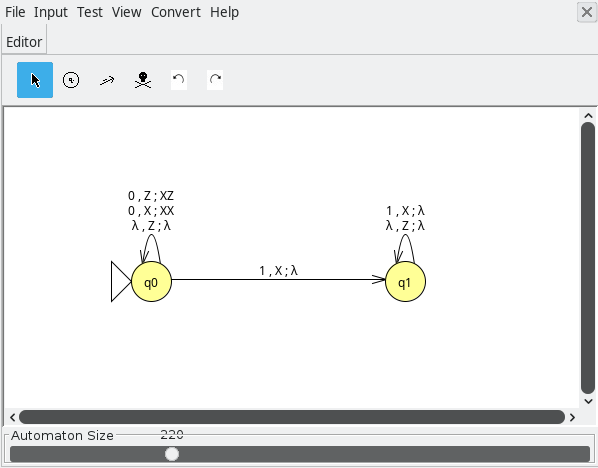
\includegraphics[scale=0.6]{jflappila}
	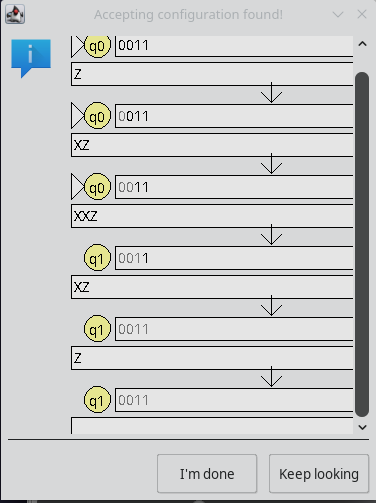
\includegraphics[scale=0.6]{jflappilaexec}
\caption{Implementación y ejecución del autómata con pila para la cadena \texttt{0011}.}
\end{center}
\end{figure}
